\section{Drive Shaft Assembly}
The drive shaft is located between the reduction shaft and the drive box. It is designed to transmit the torque from the reduction shaft to the driving sprocket located within the exterior drive box. The shaft is coupled to the reduction shaft with a flexible coupling and runs the inside of the pivot.There is a key for both ends of the flexible coupling and a set screw on the reduction shaft end. A snap ring was added to the output shaft on the coupling end to allow proper placement of the coupling along the shaft, since the set screw was not reachable once mounted in the pivot. With the pivot being over built to reduce as much deflection as possible at this point it allowed for the output shaft to experience minimal bending moments under loading. The output shaft consists of a bushing for the sprocket, a 3/16" key slot on the reduction end, 3/8" key slot at the sprocket bushing, two taper roller bearing bearings which were located in the cape and the other in the pivot itself and two shaft mounted seals. Figure~\ref{fig:output_shaft} shows the output shaft with the taper roller bearings mounted, shaft seals mounted and the grove for the snap ring at the end that has the flexible coupling attached. The output shafts were manufactured with 1045 steel which was suggested by Penguin ASI since spare material was available in the facility.
\begin{figure}[htbp]
	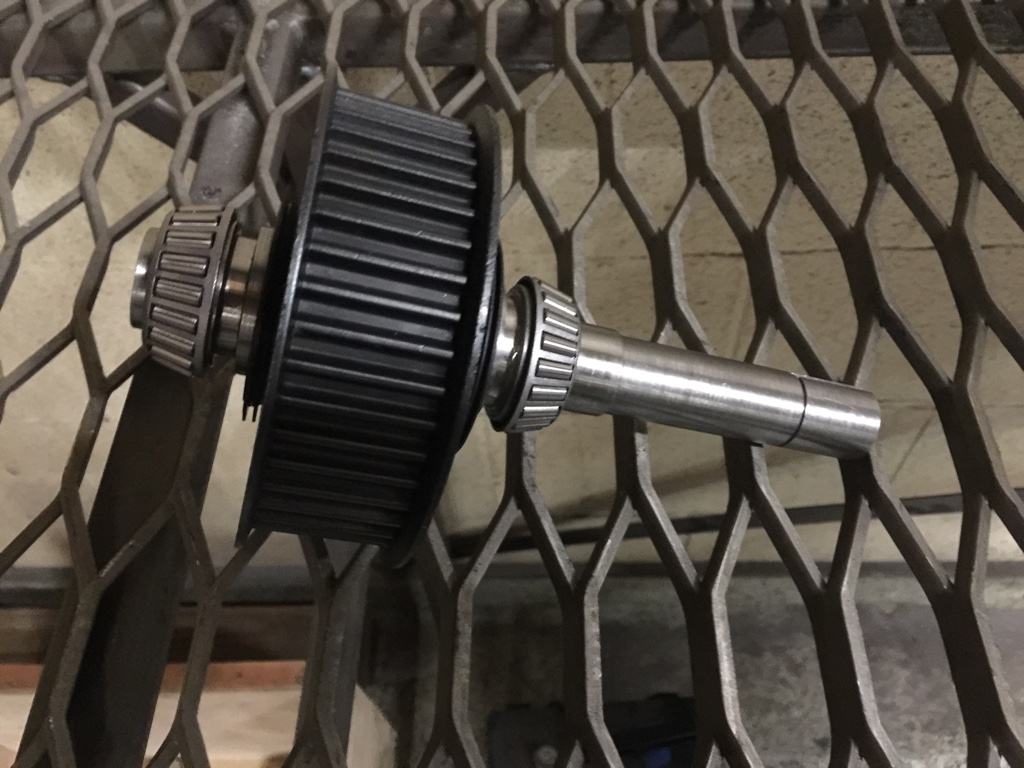
\includegraphics[width=\linewidth]{images/drive_shaft_assembly_bld.jpg}
	\caption{Assembly of output shaft with bearings, seals and sprocket mounted.}
	\label{fig:output_shaft}
\end{figure}
\subsection{Design Constraints and Functional Requirements}
The design of the output shaft had a length constrained to the distances between the reduction shaft and the end of the exterior drive box. It was required to transmit the torques and withstand the radial forces that can be seen in Table~\ref{tab:output_shaft_specs}.   

\subsection{Analysis and Design}
Using the DE-Goodman equation the minimum diameter of the output shaft was able to be calculated after two iterations. The minimum shaft diameter ended up being 20 mm and the bearings were selected using the SKF manual to select the proper taper roller bearings for the loading conditions that can be seen in Figure~\ref{fig:fb_output_shaft}. The free body diagram for the shaft is only the end that contains the two taper roller bearings and the bushing for the sprocket since the coupling end is assumed to be rigid.The finite element analysis for the output shaft can be seen in the appendix.
\begin{figure}[H]
	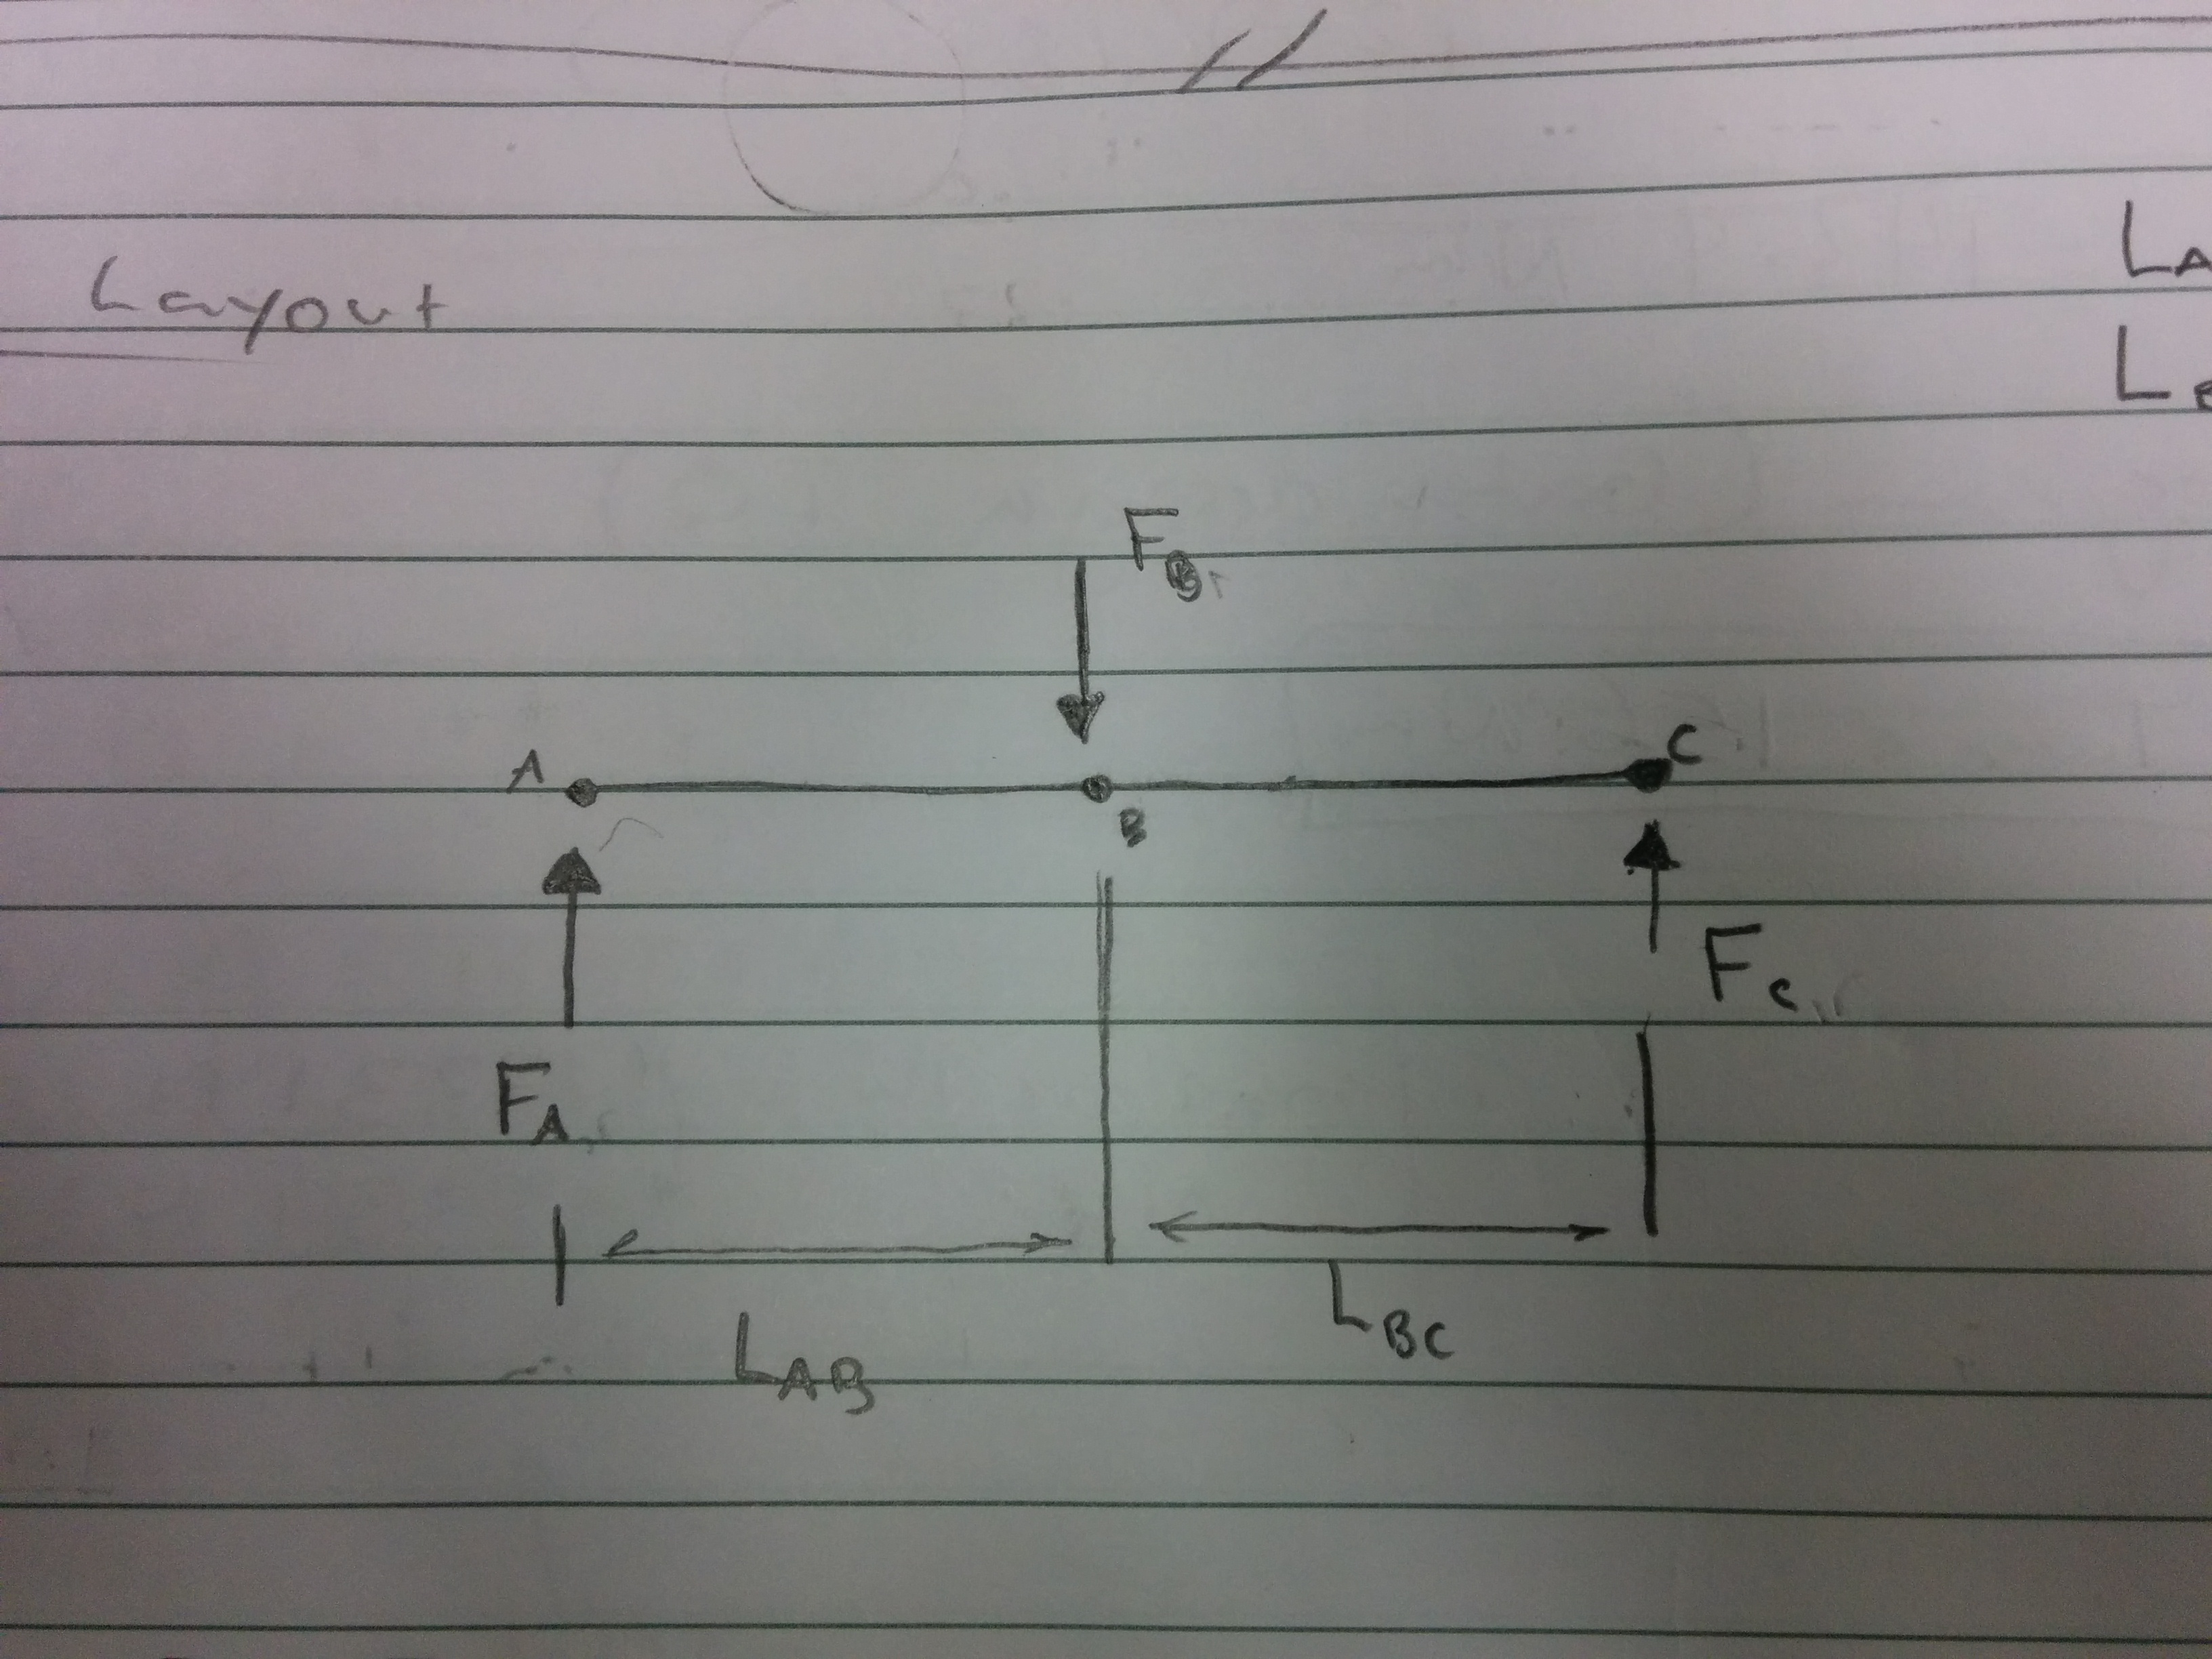
\includegraphics[width=\linewidth]{images/fb_output_shaft.jpg}
	\caption{Free Body Diagram for Output Shaft.}
	\label{fig:fb_output_shaft}
\end{figure}
\begin{table}[H]
	\centering
	\caption{Output Shaft Design Specifications}
	\begin{tabular}{| p{5cm}llp{7cm} |} \hline
		Requirement & Value & Unit & Reason \\ \hline
		Torque Transmission & 156 & Nm & Max torque transmitted by motor to the driveshaft assuming operation at 895.2\,W through a 30:1 reduction \\
		Radial Load & 3331	& N & Radial load applied by drive sprocket \\ \hline
	\end{tabular}
	\label{tab:output_shaft_specs}
\end{table}

